\documentclass[twocolumn]{emulateapj}
\usepackage{natbib}
\usepackage{comment}
\newcommand{\vdag}{(v)^\dagger}
\def\ba{\begin{eqnarray}}
\def\ea{\end{eqnarray}}
\usepackage{graphicx, amsmath, amsthm, amssymb,color}
\newcommand\aastex{AAS\TeX}
\newcommand\latex{La\TeX}
\def\qr#1{{\color{red}{\bf Cristobal: #1}}}
\def\ekd#1{{\color{green}{\bf Emily: #1}}}
\def\cc#1{{\color{blue}{\bf CH: #1}}}

\shorttitle{Imprints of outer giant planets on Close-in super-Earths}
\shortauthors{Diebert et al.}

\begin{document}


%%%%%%%%%%%%%%%%%%%%%%%%%%%%%%%%%%%%%%%%%%%%%%%%%%%%%%%%%%%%
% TITLE %
%%%%%%%%%%%%%%%%%%%%%%%%%%%%%%%%%%%%%%%%%%%%%%%%%%%%%%%%%%%%
\title{Dynamical imprints of outer giant planets on Close-in super-Earths}

%%%%%%%%%%%%%%%%%%%%%%%%%%%%%%%%%%%%%%%%%%%%%%%%%%%%%%%%%%%%
% AUTHOR %
%%%%%%%%%%%%%%%%%%%%%%%%%%%%%%%%%%%%%%%%%%%%%%%%%%%%%%%%%%%%
\author{Emily Deibert\altaffilmark{1,2},Chelsea Huang\altaffilmark{1,3} \&
Cristobal Petrovich\altaffilmark{2,3}}

\altaffiltext{1}{Dunlap Institute for Astronomy \& Astrophysics, University of Toronto, 50 St. George Street, Toronto, Ontario, M5S 3H4, Canada}
\altaffiltext{2}{Canadian Institute for Theoretical Astrophysics, University of Toronto, 60 St. George Street, Toronto, Ontario, M5S 1A7, Canada} %\email{cpetrovi@cita.utoronto.ca}
\altaffiltext{3}{Centre for Planetary Sciences, Department of Physical \& 
Environmental Sciences, University of Toronto at Scarborough, Toronto, 
Ontario M1C 1A4, Canada}

%%%%%%%%%%%%%%%%%%%%%%%%%%%%%%%%%%%%%%%%%%%%%%%%%%%%%%%%%%%%
% ABSTRACT %
%%%%%%%%%%%%%%%%%%%%%%%%%%%%%%%%%%%%%%%%%%%%%%%%%%%%%%%%%%%%
\begin{abstract}


The hundreds of multi planetary systems discovered by the \textit{Kepler} mission are typically observed to reside in close-in ($\lesssim0.5$ AU) orbits and with low eccentricities and low mutual inclinations.
We run N-body experiments to study the effect that  initially unstable  outer ($\gtrsim1$ AU) non-transiting giant planets, whose end orbital states resembles those of the systems discovered by Radial Velocity surveys, can have on the orbital configurations of these close-in multi transiting super-Earths.  
Our experiments show that the main effect of the outer giant planets on the ensembles of three close in super-Earths are:
(i) to reduce their multiplicity (by a factor of xx);
(ii) to excite their eccentricities at levels that 
anti-correlate with the multiplicity;
(iii) to excite their inclinations relative to the 
initial orbital plane, but not their mutual inclinations.
As a result, our model predicts the existence of a population of dynamically hot single transiting planets with eccentricities of $\sim 0.3-0.4$ (quote range or mean?) and inclinations $\sim 20-30^\circ$, possibly explaining existing eccentric super-Earths discovered by Radial Velocity surveys such as HD\,125612c, the 
recent eccentricity measurements of \textit{Kepler} super-Earths from transit durations 
and the tentative observation that single transiting systems have a wider distribution of stellar obliquities compared to the multi transiting systems.
Future observations from TESS will reveal more of these hot population of single transiting planets, and follow up radial velocity studies could be able to
to test our models and see whether they have outer giant planets.


\end{abstract}

%%%%%%%%%%%%%%%%%%%%%%%%%%%%%%%%%%%%%%%%%%%%%%%%%%%%%%%%%%%%
% KEYWORDS %
%%%%%%%%%%%%%%%%%%%%%%%%%%%%%%%%%%%%%%%%%%%%%%%%%%%%%%%%%%%%
\keywords{planets and satellites: dynamical evolution and stability}

%%%%%%%%%%%%%%%%%%%%%%%%%%%%%%%%%%%%%%%%%%%%%%%%%%%%%%%%%%%%
% INTRODUCTION %
%%%%%%%%%%%%%%%%%%%%%%%%%%%%%%%%%%%%%%%%%%%%%%%%%%%%%%%%%%%%
\section{Introduction} \label{sec:intro}

Originally launched in 2009, NASA's \textit{Kepler} mission \citep{Borucki2010} is responsible for the discovery of thousands of planetary candidates, including over 3000 confirmed planets (e.g., \citealt{Mullally2015,Burke2015,Morton2016}). Through monitoring periodic changes in brightness of light curves from stars (i.e. the ``transit method''), \textit{Kepler} is able to detect planets with radii on the order of 1 $\text{R}_{\oplus}$, although the majority of planets detected are so-called ``super-Earths'' or ``sub-Neptunes'' (with radii $\sim 1.2 - 3 \text{R}_{\oplus}$ \citep{Burke2015}). Of the thousands of planetary systems discovered by \textit{Kepler} to date, $80\%$ are single-transit systems (i.e. only one planet is observed to transit), while the other $\sim20\%$ consist of 2-7 transiting planets (\citealt{Mullally2015}). 


The multiple planet systems in the \textit{Kepler} sample populate dynamically cold orbits with low eccentricities and mutual inclinations ($e,i_{\rm m}\ll1$). 
In particular, the eccentricities derived from transit timing variations (TTVs) are typically $\sim0.01$ \citep{Wl13},
while the transit durations of ensembles of multi transiting planets can be well-fitted with a Rayleigh distribution (Equation \ref{eq:sigma_e}) with mean values of $\bar{e}\sim0.04$ \citep{VA15,xie16} 
and  $\bar{i}_{\rm m}\simeq1-2^\circ$ 
\citep{FM2012,Fabrycky2014}.

In contrast, the properties of the single-transit planet systems seem to be much less certain. 
\citet{Lissauer2011} first noted with preliminary {\em Kepler} data that when modeling the mutual inclination distribution as a Rayleigh function,
they had difficulty fitting the large observed ratio of single-transiting systems to multiple-transiting systems. This ``problem" is later on referred to as the ``\textit{Kepler} dichotomy'' in several other studies (\citealt{Johansen2012,HM13,Ballard2016}). 
A wide range of studies into this problem have been undertaken with varying degrees of success \citep[e.g.,][]{Johansen2012,Moriarty2015,Ballard2016,Dawson:2016}, but a consistent picture is still needed. 

This dichotomy might not only be reflected on the derived occurrences between single and multis, but there is tentative evidence that at least a fraction of the single transiting planets in \textit{Kepler} occupy dynamically hotter orbits.
In particular, \citet{xie16} find that the best fit to the transit durations of single transiting planets is achieved by invoking either a single Rayleigh distribution with  $\bar{e}\simeq0.28$ or two independent Rayleigh distributions where $\sim 80\%$ of the systems have $\bar{e}\sim0.04$ (similar to the multi transiting systems above) and the remaining $\sim20\%$ have $\bar{e}\sim0.5$.
Similarly, by combining measurements of the star's rotation period, radius, and projected rotational velocity, \citet{MW14} found some evidence that multi transiting systems to have lower stellar obliquities than
their single transiting counterparts, which can be indicative of larger individual inclinations in the singles assuming that the invariable plane nearly coincides with the host star's equator.

A dozen of these dynamically hot close-in super-Earth/Neptune systems are also seen in the Radial Velocity surveys, often with giant planets companion further out ($a>1\,AU$). As show in Figure \ref{fig:observed}, these inner super-Earths (defined as $M\sin i<0.1 M_J$) can easily have reported eccentricity of about $\sim0.1-0.4$. For example, HD\,125612c ($P\sim4$\,day, $Msini\sim18\,M_{\odot}$) was determined to have an eccentricity of $0.27\pm0.12$ \citep{LoCurto:2010}. 


In this paper, we put forth a connection between these dynamically ``hot" super-Earths and distant giant planets. We propose a scenario by which scattering between distant planets with properties drawn from Radial Velocity surveys can robustly introduce single, eccentric super-Earth systems, and therefore account for the observed 
differences between single- and multi-transit systems observed in \textit{Kepler} data. 

%It is hence worth exploring, are these radial velocity super Earths part of the ``bizzare" \textit{Kepler} singles? How would the scattering process formed the radial velocity giant planets and the later on dynamical interaction between the giant planets and these Super Earths shape the planet system architectures different from those of the typical Kepler multies? 



%A wide range of studies into the \textit{Kepler} dichotomy have been undertaken with varying degrees of success. For example, \cite{Johansen2012} find that planetary instability of triple gas-giant systems can explain the \textit{Kepler} dichotomy. In a later study, \cite{Moriarty2015} proposed that the \textit{Kepler} dichotomy is naturally explained by planetary formation within planetary disks of varying surface density profiles. Furthermore, they find evidence that the \textit{Kepler} dichotomy varies with stellar type. In another paper, \cite{Ballard2016} find that the \textit{Kepler} dichotomy is best explained by a ``mixture model'' in which approximately half of all systems are either single or contain multiple planets with large mutual inclinations, while the other half contain approximately 7 planets with mutual inclinations of approximately 2\,$^{\circ}$.

%Our methods involve drawing from observations of both \textit{Kepler} and RV planets in order to simulate systems consisting of a closely-packed (i.e. within 1 AU) inner system of super-Earths and a more distant (i.e. between 2-5 AU) system of Jupiter-like planets. Using the N-body code REBOUND (\citealt{Rein2011}), we evolve a statistically-significant number of such systems over time and report on the mutual inclinations and number of transits of the evolved systems. We furthermore investigate the results of evolving each population (i.e. super-Earths and Jupiter-like planets) separately, and incorporate the effects of general relativity into our simulations.

This paper will proceed as follows. In section \ref{sec:sims}, we will discuss the details of the code used to run the simulations, as well as the initial conditions chosen to explore the problem. Our results are presented in section \ref{sec:results}, including the effects of different populations and initial conditions used in the simulations. 
During the course of this work, many authors explored various interaction between giant planets and close-in super-Earths \citep[e.g.][]{Lai2016,GF16,hansen2016}. We discuss our result together with these works in section \ref{sec:discussion}, and our conclusions are presented in section \ref{sec:conclusion}.  



\begin{figure}[htbp!]
\centering
\includegraphics[width=\columnwidth]{observed_try3.png}
\caption{Known planet systems (from exoplanets.org) with long period giant planets and close-in super-Earths ($M{\rm sin}i<0.1\,M_{J}$), color coded by the number of planets in the system. The size of the markers are proportion to $M{\rm sin}i^{1/3}$. The planet systems we used in this figure including 55 Cnc \citep{Fischer:2008}, BD -08 2823 \citep{Hebrard:2010}, GJ\,832 \citep{Wittenmyer:2014}, GJ\,876 \citep{Correia:2010}, HD\,11964 \citep{Wright:2009}, HD\,125612 \citep{LoCurto:2010}, HD\,181433 \citep{Bouchy:2009}, HD\,190360 \citep{Courcol:2015}, HD\,215497 \citep{LoCurto:2010}, HD\,47186 \citep{Bouchy:2009}, HIP\,57247 \citep{Fischer:2012}, Kepler-68 \citep{Marcy:2014}, Kepler-89 \citep{Weiss:2013}, mu Ara \citep{Pepe:2007}.  
\label{fig:observed}}
\end{figure}

%\clearpage


\section{Simulations}
\label{sec:sims}
We run N-body simulations of the evolution of the orbits of inner \textit{Kepler}-like planets and outer giant planets (masses $>0.3M_J$) orbiting a solar-type star. 
Planet–star and planet-planet collisions are assumed to result in momentum-conserving mergers with no fragmentation. Collisions are assumed to happen when the distance between two planets (or a planet and the star) becomes less than the sum of their physical radii. The merged body is assumed to conserve total mass and volume. 
A planet is ejected from the system when the distance from the center of mass exceeds 100\,AU and the eccentricity is larger than 1, or when the distance from the center of mass exceeds 1000\,AU. 


\subsection{The code}
\label{sec:code}

We use the publicly available integrator IAS15 
\citep{RS15}, which is a high-order scheme
that is part of the REBOUND package \citep{Rein2011}.
 We justify this choice because we 
are mostly interested in the evolution of dynamically-active 
systems where planets experience several close encounters, and 
the IAS15 integrator can handle close encounters with
high precision.

We include the effects from General Relativity in some 
experiments using the package REBOUNDx with the option 
{\it gr-potential} (Tamayo et al., in prep.), which gives 
the right pericenter precession, but gets mean motion wrong by 
$\mathcal{O}(GM/[ac^2])$.


%%%%%%%%%%%%%%%%%%%%%%%%%%%%%%%%%%%%%%%%%%%%%%%%%%%%%%%%%%%%
% INITIAL %
%%%%%%%%%%%%%%%%%%%%%%%%%%%%%%%%%%%%%%%%%%%%%%%%%%%%%%%%%%%%
\subsection{Initial conditions}
\label{sec:init}
%{\bf TBD: divided up}

We first initialize our planetary systems with either super-Earths (the \textit{Kepler} population) or gas giant planets (Radial Velocity population) so we can match the bulk of their orbital architectures after either population has evolved for $>1$ Myr. We assess the match to the observed orbital properties for the \textit{Kepler}-like systems and the Radial Velocity population in \S\ref{sec:kepler} and \ref{sec:jupsonly}, respectively.

\subsubsection{Super-Earth population}

We initialize three Super-Earths located inwards of $\sim 1\,$ AU
and in long-term stable orbits. 
We choose their semi-major axes from the fitting function for the probability distribution of semi-major axes in the {\it  Kepler} sample, after accounting for geometric selection effects \citep{TD11}: 
\ba 
dp(a)=0.656 \frac{(a/a_0)^{3.1}} {1+(a/a_0)^{3.6}}
\frac{da}{a}, 
\label{eq:epsilon}
\ea 
where $a_0=0.085\,$AU and the semi-major axes are restricted to
$ a<1.15\,\mbox{AU}$.
We draw three independent random values from this distribution
and compute the period ratio between neighboring planets $\mathcal{P}$
as
\ba
\mathcal{P}=\left(a_{i+1}/a_{i}\right)^{3/2},
\ea
 where $i$ is in order of increasing semi-major axes.
We further limit the period ratio between any outer planet and its neighboring inner planet to be $1.4<\mathcal{P}<5$. 
The super-Earths can become unstable in timescales comparable to the ages of the systems by themselves at $\mathcal{P}<1.4$\footnote{For reference, an evenly-spaced three-planet system can remain stable for $\gtrsim10^{9}$ orbits
when their mutual separations are $\gtrsim10R_{H}$, which corresponds
to period ratios of $\gtrsim1.4$ for $10M_\oplus$ planets(reference!!). }, while too widely-separated planet pairs ($\mathcal{P}>5$) can be easily destabilized by outer giant planets.
The distribution of period ratios between neighboring planets are shown in Figure \ref{fig:init-pratio} and we observe that it roughly matches the observed one from \textit{Kepler}. We note that the observed distribution has not been corrected for the effect of geometric transit probability, therefore it has an excess at the end with shorter period ratios.  


The planets have non-zero eccentricities $e$
and inclinations $i$. These are assumed to be randomly distributed following a Rayleigh law, 
\ba
dp=\frac{x\,dx}{\sigma_x^2} \exp\left(-\onehalf x^2/\sigma_x^2\right),
\label{eq:sigma_e}
\ea
where $x=e$ or $i$ and $\sigma_x$ is an input parameter that
is related to the mean and rms eccentricity or inclination by $\langle
x\rangle=\sqrt{\pi/2}\sigma_x=1.253\sigma_x$, $\langle
x^2\rangle^{1/2}=\sqrt{2}\sigma_x=1.414\sigma_x$.


 The masses of the super-Earths were either 5, 10, or 15 $\text{M}_{\oplus}$, but the ordering of the masses was randomized. This choice is arbitrary and the range of masses $5-15~\text{M}_{\oplus}$ is characteristic for planets with $\sim2-4~\text{R}_{\oplus}$ (e.g., \citealt{WM14}).
 

\subsubsection{The gas giant population}

We choose the semi-major axis to be uniformly distributed 
in a defined range 2-5 AU. 
Labeling the planets by subscripts $i$ in order of increasing 
semi-major axis, we impose a minimum initial spacing 
of the orbits given by
\ba
\Delta a_{i,i+1}&\equiv& a_{i+1}-a_{i}>K R_{H,i,i+1},\mbox{where} \nonumber \\
R_{H,i,i+1}&=&\left(\frac{M_i+M_{i+1}}{3 M_\star}\right)^{1/3}
\frac{a_i+a_{i+1}}{2},
\label{eq:delta_a}
\ea
and $R_{H,i,i+1}$ is the mutual Hill radius of planets
with masses $M_i$ and $M_{i+1}$.

The initial spacing between orbits mainly changes the 
timescale of onset of dynamical instability
(e.g., \citealt{CWB96}). 
Our choice of $K$ in Equation (\ref{eq:delta_a}) is
empirically guided by the fact that we would like to avoid very 
closely-packed systems which might be subject to gravitational focusing, leading to a spurious excess of planet-planet collisions. 

We initialize the system with three gas giant planets
and use $K=3$.
For reference, a crude estimate of the instability time
can be obtained from the numerical experiments by  
\citet{CFMS2008} using a different initial spacing law $\Delta a_{i,i+1}=\tilde{K} R_{H,i,i+1}$ 
(i.e., the spacing is a fixed multiple of the Hill radius, rather than 
exceeding a multiple of the Hill radius). 
They show that for a distribution of planet masses in the
range $0.4-4~M_J$ the median instability 
timescale can be fitted by the following expression:
\ba
\log_{10} (t/\mbox{orbits})=0.021+0.03\exp(1.1~\tilde{K}),
\label{eq:K_tilde}
\ea
where the orbits are those of the innermost planet. 
By assuming that the spacing is a fixed multiple of the Hill radius and that the planet have Jupiter 
masses, our range of semi-major axes of $2-5$ AU allows for $\tilde{K}$ in the range $\sim 3-5$  meaning instability timescales spans in 
$\sim10-10^7$ orbits. In practice, our experiments 
show that most (96$\%$) systems become unstable within 1 Myr (see the results in \S\ref{sec:jupsonly}). 

The masses of the Jupiters are uniformly drawn between 0.3 $M_{\rm J}$ and 3 $M_{\rm J}$. These initial conditions are chosen so that our Jupiter like planets will reproduce the bulk of the eccentricities and semi-major axes of the radial velocity population (see Section \S \ref{sec:jupsonly}). 


\begin{figure}[htbp!]
\includegraphics[width=\columnwidth]{SEOnly/SEonly_a.pdf}
\includegraphics[width=\columnwidth]{SEOnly/SEonlyPratio.pdf}
\caption{The top panel shows the initial semimajor axis distribution of the super-Earths. The bottom panel shows the initial (black and hatched) and end (red) period ratio distribution of neighboring super-Earths. To compare with, we overplotted the period ratio of nearest neighbour for the \textit{Kepler} three planet systems from release DR24 \citep{Coughlin:2016}.  
\label{fig:init-pratio}}
\end{figure}



%Fig. \ref{fig:mass-init} shows the initial setup of the randomized-mass simulations.

%\begin{figure}[htbp!]
%\includegraphics[width=\columnwidth]{Initial.pdf}
%\caption{The initial plot of orbital eccentricity vs semi-major axis, colour-coded by mass, for the set of simulations where the planets' masses have been randomized.}
%\label{fig:mass-init}
%\end{figure}

%{\bf TBD: need a schematic figure to demonstrate the initial set ups}

%CH: initial condition not important to show
%\begin{figure}[htbp!]
%\centering
%\includegraphics[width=\columnwidth]{newinc-initial.pdf}
%\caption{The initial orbital eccentricity vs semi-major axis for the six planets run.}
%\label{fig:init-e}
%\end{figure}

%\begin{figure}[htbp!]
%\includegraphics[width=\columnwidth]{newinc-initial-inc.pdf}
%\caption{The initial nclination vs semi-major axis for the six planets run.}
%\label{fig:init-i}
%\end{figure}

\begin{figure}[htbp!]
\centering
\includegraphics[width=\columnwidth]{a_e_jup_only.pdf}
\caption{Eccentricity versus semi-major axis of the Jupiter-like planet at the end of 1\,Myr evolution. The planets are colour-coded by the multiplicity of their system.}
\label{fig:mass-final}
\end{figure}



\begin{figure}[htbp!]
\centering
\includegraphics[width=\columnwidth]{ejup_only.pdf}
\includegraphics[width=\columnwidth]{inc_jup_only.pdf}
\caption{The final cumulative eccentricities (upper panel) and inclinations (lower panel) distribution of the Jupiter like planets within 5\,AU after 1\,Myr evolution (black line). Red line indicate the cumulative eccentricity distribution of planets detected by radial velocity method with $a<5\,AU$.
The initial eccentricity and inclination distribution of our simulation has a Rayleigh width of $\sigma_e=0.01$ and $\sigma_i=0.01$.
\label{fig:hist-jup-only}}
\end{figure}


%\begin{figure}[htbp!]
%\centering
%\includegraphics[width=\columnwidth]{inc_jup_only.pdf}
%\caption{The final inclination distribution of the Jupiter like planets within 5\,AU after 1\,Myr evolution.
%The initial inclination distribution has a Rayleigh width of $\sigma_i=0.01$.
%}
%\label{fig:hist-inc-jup}
%\end{figure}



\section{Results}
\label{sec:results}
\subsection{Kepler-like systems only}
\label{sec:kepler}

We evolved 158 systems of 1 Myr. We find no significant change on the multiplicity and orbital elements $e$ and $i$ ($\sigma_e$,$\sigma_i$\,$\sim0.01$). 
The distribution can roughly reproduce the spacing and typical eccentricities \citep{Fabrycky2014}. 

The results are expected because the typical mutual Hill spheres have $\sim0.005$ AU and $\sim10$ mutual Hill separations required for stability up to $10^8$ orbits (citations) correspond to
period ratios $\lesssim1.6$, where we have only a small fraction of the systems.

\subsection{The radial velocity population only}
\label{sec:jupsonly}


\begin{table}[htbp!]
\centering
\begin{tabular}{c  c}
\hline
\hline
$\text{N}_{\text{J}}$ & Percentage of Systems (\%) \\
\hline
1 & 19 \\
2 & 76 \\
3 & 4  \\
\hline
\end{tabular}
\caption{Multiplicity distribution of the Jupiter like planets.\label{tab:randommass}}
\end{table}

We evolve 160 realizations of systems for 1\,Myr. 
The fraction of systems with a given final number of planets is shown in Table \ref{tab:randommass}, where we observe that most systems ($\sim80\%$) end up with two planets (also see in Figure \ref{fig:mass-final}). 
The prevalence of two-planet systems is also observed in other similar scattering experiments of three giant giant planets
(e.g., \citealt{CFMS2008,Johansen2012,PTR14}). 
With radial velocity follow up and AO imaging, \citet{Knutson14,bryan16} estimated that about half of the cold giants in their survey have companions. 
Only $\sim5\%$ of the systems stay relatively inactive, which are expected to become unstable if were evolved for long enough time.

%From Figure \ref{fig:mass-final} and Table \ref{tab:randommass},
%we observe
%that most of systems become unstable, in particular, about 76$\%$ of the systems lost one of its planet at the end of run. About $20\%$ of the systems have only one planet left, due to one collision between the planets with either an ejection or collision with the host star. 

We show the eccentricity distribution of giant planets with $a<5$\,AU in Figure \ref{fig:hist-jup-only}, which can be directly compared to the Radial Velocity. 
The mean and median eccentricities of these systems are 0.31
and 0.24, which reproduce the observed value of $\simeq 0.26$ and $0.2$ of planets at $>1$\,AU. 
This is not a coincidence as we have tuned the range of the mass distribution and used $0.3-3M_J$ to explain the observe eccentricities\footnote{The resulting eccentricities after scattering of two planets decreases as their mass ratio $\max\{m_1/m_2,m_2/m_1\}$ increases \citep{Ford2008}.}.

Most of the systems have relatively low inclinations, with a mean and median inclination of $\sim 12.7^\circ$ and    $\sim6^\circ$, respectively (Figure \ref{fig:hist-jup-only}). 

%cite knutson et al 2014 and Bryan et al. 2016: cold Jupiters have outer companions...

%CH: does not need the final mass figures. 
%\begin{figure}[htbp!]
%\centering
%\includegraphics[width=\columnwidth]{Final-Mass.pdf}
%\caption{The final eccentricities vs semi-major axes of the surviving planets. Planets are colour-coded by their masses.}
%\label{fig:mass-final-mass}
%\end{figure}







%CH: we can use the table only for this:
%\begin{figure}[htbp!]
%\includegraphics[width=\columnwidth]{NJupiters.pdf}
%\caption{A histogram of the number of planets remaining in the 160 simulated systems after 1 Myr of integration. Note that these are the systems for which the initial masses of the planets were randomized.}
%\label{fig:mass-histogram}
%\end{figure}

\begin{figure*}[htbp!]
%\includegraphics[width=\columnwidth]{newinc-multiplicity.pdf}
\includegraphics[width=0.9\columnwidth]{Fiducial/a_e_nplanet_458.pdf}
%\caption{Orbital eccentricity vs semi-major axis for the fiducial run, color-coded by system multiplicity. Jupiter like planets are represented by circles, while Super Earths are represented by diamonds.}
%\label{fig:multiplicity}
%\end{figure}
%\begin{figure}[htbp!]
%\includegraphics[width=0.9\columnwidth]{newinc-nearths.pdf}
\includegraphics[width=0.9\columnwidth]{Fiducial/a_e_nearth_458.pdf} \\
%\caption{Similar to Figure \ref{fig:multiplicity}, while the planets are color coded by the number of Super Earths in the system.}
%\label{fig:nearths}
%\end{figure}
%\begin{figure}[htbp!]
%\includegraphics[width=0.9\columnwidth]{newinc-njupiters.pdf}
\includegraphics[width=0.9\columnwidth]{Fiducial/a_e_njup_458.pdf}
%\caption{Similar to Figure \ref{fig:multiplicity}, while the planets are color coded by the number of Jupiters in the system.}
%\label{fig:njupiters}
%\end{figure}
%\begin{figure}[htbp!]
\includegraphics[width=0.9\columnwidth]{Fiducial/a_i_nearth_458.pdf}
\caption{
Orbital eccentricity vs semi-major axis for the fiducial run, color-coded by system multiplicity (top left panel), number of super-Earths (top right panel) and number of giant planets (bottom left panel) in the system. 
Bottom right panel shows orbital inclination vs semi-major axis for the fiducial run, color-coded by number of super-Earths in the system.
Jupiter like planets are represented by circles, while super-Earths are represented by diamonds.}
\label{fig:results}
\end{figure*}

%%%%%%%%%%%%%%%%%%%%%%%%%%%%%%%%%%%%%%%%%%%%%%%%%%%%%%%%%%%%
% RESULTS %
%%%%%%%%%%%%%%%%%%%%%%%%%%%%%%%%%%%%%%%%%%%%%%%%%%%%%%%%%%%%
\subsection{The super-Earth and gas giant populations together} \label{sec:standardrun}

Having characterized both the \textit{Kepler} and Radial Velocity populations independently, we now turn to our main experiment, namely putting both populations together.

We first describe the results for our fiducial simulation. In this simulation we set up systems with initially 3 super-Earths and 3 Jupiters, while the 
eccentricities and inclinations of all the planets were drawn from Rayleigh distribution in Equation (\ref{eq:sigma_e}) with $\sigma_e=0.01$, and $\sigma_i=0.01 \,{\rm rad}$. 

We evolve the fiducial run for 527 realizations till 1\,Myr. The outcomes are listed in Table \ref{tab:results}.
Figure \ref{fig:results} shows the eccentricity versus semi-major axis of all the remaining planets at the end of 1\,Myr, color-coded by system multiplicity, number of remaining super-Earths, number of remaining Jupiters, respectively. It also shows the inclination versus semi-major axis of all the remaining planets at the end of 1\,Myr, color coded by number of remaining super-Earths. We detailed the various outcomes as the following: 

\begin{itemize}
\item {\bf No super-Earths:} slightly less than half of the system ($47 \%$) resulted in that the scattering of giant planets disrupt the inner super-Earths completely, leaving mostly two eccentric Jupiter like those in typical RV systems. 

\item {\bf super-Earths with Giant planets:} most of the other half ($49\%$) of the systems lost at least one giant planet due to either ejection or scattering, stir up the close-in super-Earths but do not destroy all of them.
\begin{itemize}

\item The systems with one, two and three super-Earths remaining together with two giant planets are about 16, 3, and 14 percent of the total outcomes. The remaining single super-Earths almost always have high eccentricity and inclination. They typically have a flat eccentricity distribution from 0.1 to as high as 0.8, and inclination as high as 60 degrees. The systems with two super-Earths remaining have eccentricity between 0.1-0.4. A fraction of the three super-Earths systems have modest eccentricity between 0.1-0.2, and inclination between 10-20 degree. If a collision happen between the giant planets instead of an ejection, the super-Earths remain dynamically cold. 

\item About $7\%$ of the systems have one eccentric Jupiter left with dynamically hot super-Earths systems. Since the eccentricity distribution of the single Jupiter is similar to those of the inner planet of the two Jupiter systems, the properties of super-Earths are almost indistinguishable from those have two Jupiters.

\end{itemize}

\item {\bf Inactive:} only $3\%$ have all six planets at the end of run. These systems are expected to become unstable in longer time scale. 

\end{itemize}



We take a more detailed look at the systems that lost at least one planet and still with super-Earths remaining. The inclinations and eccentricities of the systems with one/two/three super-Earths are shown in Figure \ref{fig:inc_earthonly}. 
%They follow the trend of xxx. 
In general, systems with less super-Earths have higher eccentricity and higher inclination. We show the comparison of our systems to the \textit{Kepler} single and multiple systems. 
As derived by \citet{xie16}, the \textit{Kepler} single planet systems can be modeled by an eccentricity distribution with Rayleigh width $\sigma_e=0.32\pm0.023$, while the multiple systems are much more circular, with an eccentricity upper limit at $\sim0.07$. We fit the eccentricity and inclination distribution for our single super-Earth population with a Rayleigh distribution, and obtain that the Rayleigh width to be $\sigma_e=0.32\pm0.05$ and $\sigma_i=(17\pm3)^{\circ}$. 
The Rayleigh width and its uncertainties is determined by bootstrapping the single planet population for 1000 realizations. 
%This is expected to be more eccentric than the observed single population since the observed population is contaminated by some of the dynamically cold multiple systems with only one planet transit. 



\begin{figure*}[htbp!]
\centering
\includegraphics[width=\linewidth]{Fiducial/mu_e_i_nearth_458.pdf}
\caption{Left panel shows mean orbital mutual inclination versus mean eccentricity for the systems with super-Earths survive, color coded by the number of super-Earths in the system. 
We show the linear trend $e=i$ and $e=2i$ to compare with. We also show the location of Kepler 
multiple systems (red square) and single systems (cyan diamond) on this plane as derived by \citet{xie16}. 
The inclination of the Kepler single systems are assumed to be the same as their derived eccentricity.
Kepler-56 system is noted as the green dot with the inclination taken from the measurement from the gravitational mode of the host star \citep{Huber:2013}, 
and eccentricity taken from the dynamic uplimit estimation from \citet{Huber:2013} assuming a low mutual inclination between the close-in planets. Note that for the three super-Earth systems we show the mean mutual inclination between the three possible pairs of planets. 
Right panel shows the mean mutual inclination of the system versus the obliquity of individual planets. The obliquity of all planets at the start of simulation is assumed to be close to 0. The color coding is the same as the left panel.  
\label{fig:inc_earthonly}
}
\end{figure*}

There are a few exceptions to this trend, with the super-Earths being roughly circular, while the inclinations are as high as 50 degrees. We have identified these systems as the class of ``misaligned multiples", such as Kepler-56, with low mutual inclinations between the super-Earths. We demonstrate the time evolution of one of this system in Figure \ref{fig:orbit_tilt}. In this example, the ejection of planet 2 at 0.2\,Myr has tilted the orbital plane of all the three super-Earths all together, leading to their inclinations oscillate between 30 to 90 degrees. 


\begin{figure*}[htbp!]
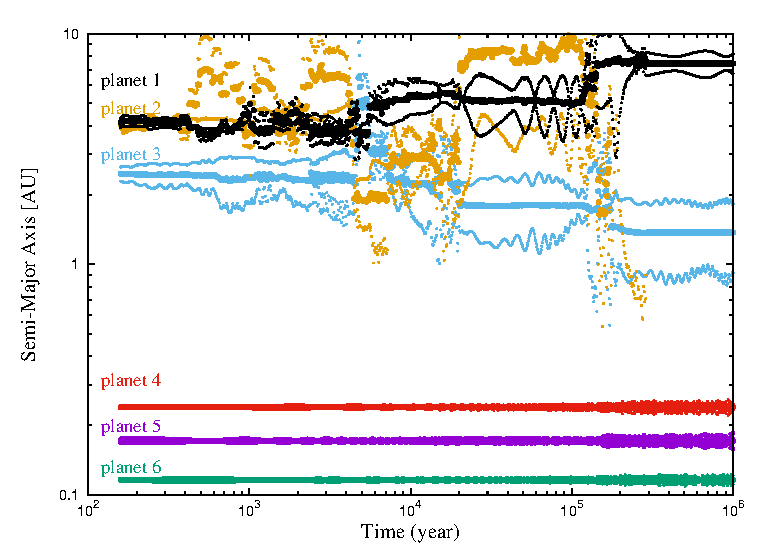
\includegraphics[width=\columnwidth]{GR/orbit_tilt_e.eps}
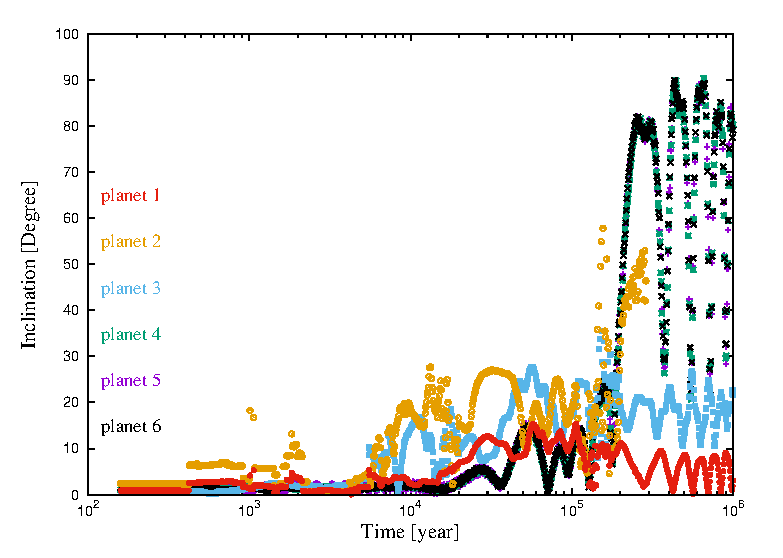
\includegraphics[width=\columnwidth]{GR/orbit_tilt_i.eps}
\caption{Time evolution of a realization of our simulation which resemble the Kepler-56 system. The left panel shows how the semi major axis (thick lines), pericenter (thin lines) and apocenter (thin lines) of 6 planets vary in 1\,Myr. The right panel shows the inclination of all the planets in degrees. One of the giant planet (planet 2) is ejected at 0.2\,Myr. At the end of 1\,Myr, This system has three roughly coplanar and circular super-Earths (planet 4,5 and 6) with two eccentric giant planets (planet 1 and 3), while the inclination of the super-Earths oscillate between 30 to 90 degrees. 
\label{fig:orbit_tilt}}
\end{figure*}


We also identified the giant planets with semi major axis smaller than 5 AU, and compare their eccentricities in Figure \ref{fig:ejup_nearth}. We report that only Jupiters with eccentricity smaller than 0.7 can keep super-Earths in the system. The lower eccentricity the Jupiters have, it is more likely to allow higher multiplicity super-Earths systems to survive. Most of the three super-Earths system are likely to be found around Jupiters with eccentricity smaller than 0.3. 

%{\bf TBD: make evolution figures for systems with one/two/three Super Earths left.}
%We demonstrate the time evolution of a xxx like system {\it CH: (a real system we like)} in Figure xxx. 





\begin{figure*}[htbp!]
\includegraphics[width=0.66\columnwidth]{Fiducial/e_jup_nearth.pdf}
\includegraphics[width=0.66\columnwidth]{Fiducial/e_jup_nearth_2Myr.pdf}
\includegraphics[width=0.66\columnwidth]{Fiducial/e_jup_nearth_10Myr.pdf}
\caption{The cumulative histogram of eccentricities for giant planets within $a<5$ AU with super-Earths in the same system. Blue, green, red and black histograms shows the result for systems with 0, 1, 2 and 3 super-Earths remaining, respectively. From left to right, we show the result simulated for 1\,Myr, 2\,Myr and 10\,Myr time. We note that the last 8\,Myr of the 10\,Myr simulations were integrated with ``whfast" integrator, while the other simulations were integrated with the higher precision ``ias15" integrator. 
\label{fig:ejup_nearth}}
\end{figure*}




\begin{comment}
\begin{table*}[htbp!]
\centering
\begin{tabular}{c c c c c c}
\hline
\hline
($\text{N}_{\text{J}}$, $\text{N}_{\text{SE}}$) & fiducial run (\%) & $\sigma_i=1^{\circ} (\%)$ & GR (\%) & 2\,Myr (\%) & 10\,Myr (\%)\\
\hline
(1, 0) & 9 & 10 & 6 & 14 & 17\\
(1, 1) & 2 & 1  & 3 & 5 & 5\\
(1, 2) & 1 & 0 & 1 & 1 & 2\\
(1, 3) & 3 & 0 & 2 & 3 & 2\\
(2, 0) & 32 & 37 & 24 & 34 & 33\\
(2, 1) & 14 & 11 & 18 & 13 & 13\\
(2, 2) & 5 & 4 & 6 & 8 & 5\\
(2, 3) & 18 & 15 & 34 & 18 & 19\\
(3, 0) & 1 & 0 & 1 & 0 & 0\\
(3, 1) & 0 & 0 & 0 & 0 & 0\\
(3, 2) & 0 & 0 & 0 & 0 & 0\\
(3, 3) & 9 &  16 & 4 &4 & 3\\
\hline

\multicolumn{4}{c}{\vspace{1cm}}\\

\hline
\hline
 & fiducial run & $\sigma_i=1^{\circ}$ & GR & 2\,Myr & 10\,Myr\\
\hline
$\bar{i}$ -- $\sigma_i $ ($^\circ$) & $27\pm4$ -- $17\pm3$ & $37\pm4$ -- $26\pm3$  & $30\pm3$ -- $22\pm3$& $27\pm3$ -- $18\pm3$ & $28\pm5$ -- $15\pm3$\\
$\bar{e}$ -- $\sigma_e$ & $0.42\pm0.04$ -- $0.32\pm0.05$  & $0.42\pm0.04$ -- $0.28\pm0.05$ & $0.43\pm0.03$ -- $0.3\pm 0.04$ & $0.44\pm0.04$ -- $0.38\pm0.05$  & $0.41\pm0.04$ -- $0.29\pm0.05$\\
\hline
\end{tabular}
\caption{Upper table: Final number of outer giant planets and super-Earths for each ensemble of integrations. Lower table:  mean and parameter $\sigma$ of the Rayleigh distribution (Equation \ref{eq:sigma_e}) of the eccentricities and inclinations of the single super-Earth systems. }
\label{tab:results}
\end{table*}
\end{comment}


\begin{table*}[htbp!]
\centering
\begin{tabular}{c c c c c}
\hline
\hline
($\text{N}_{\text{J}}$, $\text{N}_{\text{SE}}$) & fiducial run (\%)  & GR (\%) & 2\,Myr (\%) & 10\,Myr (\%)\\
\hline
(1, 0) & 9 & 6 & 14 & 17\\
(1, 1) & 2   & 3 & 5 & 5\\
(1, 2) & 1  & 1 & 1 & 2\\
(1, 3) & 3  & 2 & 3 & 2\\
(2, 0) & 32  & 24 & 34 & 33\\
(2, 1) & 14  & 18 & 13 & 13\\
(2, 2) & 5  & 6 & 8 & 5\\
(2, 3) & 18  & 34 & 18 & 19\\
(3, 0) & 1  & 1 & 0 & 0\\
(3, 1) & 0  & 0 & 0 & 0\\
(3, 2) & 0  & 0 & 0 & 0\\
(3, 3) & 9  & 4 &4 & 3\\
\hline

\multicolumn{4}{c}{\vspace{1cm}}\\

%\end{tabular}
%\caption{Architecture of resulted planet systems.}
%\label{tab:results}
%\end{table*}


%\begin{table*}[htbp!]
%\centering
%\begin{tabular}{c c c c c c}
\hline
\hline
 & fiducial run  & GR & 2\,Myr & 10\,Myr\\
\hline
$\bar{i}$ -- $\sigma_i $ ($^\circ$) & $27\pm4$ -- $17\pm3$   & $30\pm3$ -- $22\pm3$& $27\pm3$ -- $18\pm3$ & $28\pm5$ -- $15\pm3$\\
$\bar{e}$ -- $\sigma_e$ & $0.42\pm0.04$ -- $0.32\pm0.05$ & $0.43\pm0.03$ -- $0.3\pm 0.04$ & $0.44\pm0.04$ -- $0.38\pm0.05$  & $0.41\pm0.04$ -- $0.29\pm0.05$\\
\hline
\end{tabular}
\caption{Upper table: Final number of outer giant planets and super-Earths for each ensemble of integrations. Lower table:  mean and parameter $\sigma$ of the Rayleigh distribution (Equation \ref{eq:sigma_e}) of the eccentricities and inclinations of the single super-Earth systems. }
\label{tab:results}
\end{table*}




\begin{figure}[htbp!]
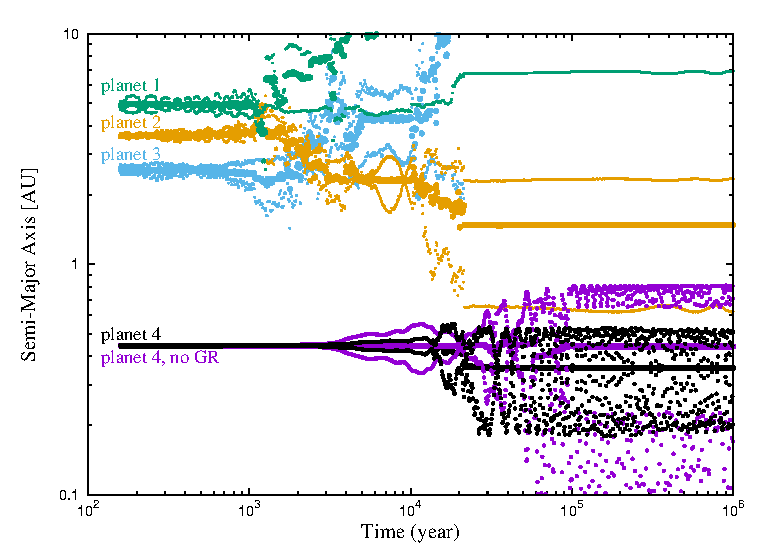
\includegraphics[width=\columnwidth]{GR/GRexample.eps}
\caption{Semi major axis (thick line), pericenter and apocenter (thin lines) of planets over time with the general relativity potential taken into account. The system start with 6 planets, with planet 1, 2 and 3 to be Jupiter like planets, and planet 4,5,6 to be close-in super-Earths. Planet 5 and 6 were ejected around $10^4$\,yrs, and are not shown in the plot. The purple curve shows the survived super-Earth (planet 4) has a modest eccentricity of about 0.4. For comparison, the green curve shows the evolution of planet 4 without the general relativity effect. The planet's eccentricity can growth to as high as 0.8 and will eventually collide with the host star without taken into account of GR.  
\label{fig:GRexample}}
\end{figure}

\subsection{Effect of General Relativity}

We include the effect that apsidal precession from general relativity has on the evolution of the super-Earths.

We simulated 160 systems with the same initial conditions as our fiducial simulations, but including  with the effect from GR precession. 
The outcomes are shown in Table \ref{tab:results} and we note that
 the overall demographics  is not changed dramatically compared to our fiducial simulation.
 Looking at the results in more detail, we note that the main effect of GR is to slightly increase the number of surviving super-Earths from from $56\%$ to $68\%$ after 1 Myr at the expense of reducing the number of systems with two giant planets and no super-Earths. This effect might be expected since the apsidal precession of the inner super-Earths can be fast enough (timescale of $\sim P_{\rm SE}\cdot(GM_\odot)/(a_{\rm SE}c^2)\sim10^5$ years, with $P_{\rm SE}$ and $a_{\rm SE}$ indicating the period and semi-major axis of the super-Earth) to quench the eccentricity excitation driven by the secular perturbations from the outer giant planets (timescale of $\sim P_{\rm SE}\cdot(M_\odot/m_J)\cdot(a_J/a_{\rm SE})^3\sim10^4-10^6$ years) that can cause the destabilization of the inner super-Earths (e.g., \citealt{MG09,WL11}).
 
 In Figure \ref{fig:GRexample}, we show one example that
illustrates how GR decreases the maximum eccentricity achieved by the single super-Earth (purples lines has no GR and black lines include GR) that survives the early scattering phase that removes the other two super-Earths and one giant planet. In this example the maximum eccentricity of the SE is $\gtrsim0.8$ without GR, while it reaches $\lesssim0.4$ when GR is included.
We caution that our calculations ignore the orbital precession due to the tidal bulges, which can have a stronger effect than GR at limiting the maximum eccentricity that the super-Earths can reach and prevent the collisions with the host star (e.g., \citealt{WL11,P15,liu15}).
 
Consistent with the expectation that GR precession can limit the eccentricity growth due to secular perturbations, we observe from Table \ref{tab:results} that the width of the eccentricity distribution of the single super-Earths decreases from 
$\sigma_e=0.32\pm0.04$ in our fiducial simulation to $\sigma_e=0.28\pm0.05$. In turn, the inclinations increase from  $\sigma_i=(17\pm3)^{\circ}$ to $\sigma_i=(22\pm4)^{\circ}$. 



%\subsection{Effect of initial mutual inclinations}

%One may wonder how much the single to multiple system ratio is determined by the initial inclination distribution. To explore this, we simulated 160 realization of the systems with the initial inclinations more spread out than our fiducial run, with $\sigma_i=1^{\circ}$ instead of 0.01\,rad. This choice is roughly the $3\sigma$ lower boundary of the mutual inclination Rayleigh width of the current {\rm Kepler} multiple planets determined by \citet{Fabrycky2014}. As show in Figure \ref{fig:transits}, the initial single to multi ratio is increased by factor of 1.25, as we would expected. The end single to multi ratio at 1\,Myr, however, didn't change much. Increase the initial inclination did increase the fraction of super-Earth systems destroyed in the simulation by $6\%$. We fitted the Rayleigh width of the eccentricity and inclination of the single planet population for this experiment. They are $\sigma_e=0.28\pm0.05$, and $\sigma_i=(26\pm3)^{\circ}$, respectively.   


\subsection{Effect of run time}

We analyse the long term stability of these super-Earths systems by extended 160 of our simulations to 2\,Myrs. As show in Table \ref{tab:results}, the fraction of systems with the super-Earths completely destroyed did not change dramatically. About 4\% more systems have been destroyed in the second million year of simulation. This is mostly due to the disturb of many of the systems with three super-Earths by eccentric giant planets. As show in Figure \ref{fig:ejup_nearth}, the eccentricity criterion for a giant planet to have three super-Earths companion reduced from 0.6 to 0.3 with the run time increase. In the meanwhile, the rate of single super-Earths kept roughly constant. The final eccentricity and inclination distribution of single super-Earths can be described by $\sigma_e=0.38\pm0.05$, and $\sigma_i=(18\pm3)^{\circ}$. 

We use the ``wfhast" integrator to continue the simulation to 10\,Myrs. 
``wfhast" is the fast and unbiased implementation of a symplectic Wisdom-Holman integrator for long term gravitational simulations \citep{ReinTamoya:2015}.  
This choice is justified because the rate of close encounter between the super-Earths have reduced dramatically in the first 2\,Myrs. Only $2\%$ more system have been destroyed, it seems that the systems reach equilibrium. This can also be observed in the eccentricity distribution of giant planets in Figure \ref{fig:ejup_nearth}. The final eccentricity and inclination distribution can be described by $\sigma_e=0.29\pm0.05$, and $\sigma_i=(15\pm3)^{\circ}$. 


\subsubsection{Number of transiting systems.}

Finally, we used the code \texttt{CORBITS} \citep{Brakensiek:2016} to determine the transit probability of super-Earths in the remaining systems. 
\texttt{CORBITS} computes the probability that any particular group of planets can 
be observed to transit in a multiple planet systems. We use bootstrap to compute the average (and 1-$\sigma$ uncertainties of) numbers of systems with single transit planet, two transit planets and three transit planets.  
The ratio between observing n transiting planets relative to n-1 transiting planets is presented in Figure. \ref{fig:transits}. From Data Release 24 of \textit{Kepler} candidates, we compute that the ratio between two planets system to single planet system is $0.21\pm0.01$, while the ratio between the three planets system to two planets system to be $0.27\pm0.04$. Our initial condition is more coplanar than the \textit{Kepler} systems, with both ratios much higher. After the systems evolved for 1\,Myr, the probabilities of observing higher multiplicity systems significantly reduced, yields ratios of $0.23\pm0.02$, and $0.39\pm0.05$. As the systems evolve further, we do not see the ratio change much. The result at the end of 10\,Myr simulation yields $0.17\pm0.03$, and $0.41\pm0.11$, which are marginally consistent with the observations. 

General Relativity allows the more of the three planets system to survive, and have higher mutual inclination (?), reduce the ratio between the three planet and two planet systems, yields ratios of $0.22\pm0.03$, and $0.31\pm0.07$, matches better with the observations. 

We note that our mechanism does not aim to explain the \textit{Kepler} dichotomy in the occurrence rate solely. Given the relatively low occurrence rate of the giant planets ($10-20\%$, \citet{Cumming:2008, Mayor:2011}), the \textit{Kepler} systems are likely to be a mixture between the perturbed and unperturbed systems.  

%As can be seen, the number of single-transit systems roughly doubles after 1 Myr of evolution of the systems. While the ratio between the two transit and three transit system stayed roughly the same, the ratio between the signal transit system and the two planet system increased to be a factor of 3.5. 


\begin{figure}[htbp!]
%\includegraphics[width=\columnwidth]{Fiducial/transitprobs-fiducial-alt.pdf}
\includegraphics[width=\columnwidth]{transprobwithinit.png}
%\includegraphics[width=\columnwidth]{Newinclination/transitprobs-onedegree-alt.pdf}
%\includegraphics[width=\columnwidth]{GR/transitprobs-gr-alt.pdf}
\caption{The ratio between the number of systems with n transiting planets relative to n-1 transiting planets. We show the result at the initial of the simulation, from the 1\,Myr, 2\,Myr and 10\,Myr evolutions with magenta diamonds, cyan triangles, blue dots, and green squares. The simulation with general relativity for 1\,Myr is show in red upper triangles. To compare with, the result from \textit{Kepler} DR24 is shown with magenta lines.
\label{fig:transits}}
\end{figure}


\section{Discussion}
\label{sec:discussion}


{\bf TBD: just brain storming conclusions right now: }

What we did: "scattering experiments that reproduce the bulk of the RV planets (eccentricities and semi-major axes)".
The main results of these experiments can be summarized as follows:

\begin{itemize}
\item  Nearly half of the inner Kepler-like systems survive the scattering events with the outer giant planets. The multiplicity of these systems is reduced: most end up having 1 planet in an eccentric and inclined orbit.

\item Data and singles: the rms (or Rayleigh fit $\sigma$) of $\psi$ and $e$.  
The fiducial run singles has $\sigma_e~0.32\pm0.05$, $\sigma_i~(17\pm3)^{\circ}$. The GR run has $\sigma_e~0.28\pm0.05$ and $\sigma_i~(26\pm3)^{\circ}$.

\item Based on our estimates of the transit probability for the simulated systems we observed that ratio between the number of the single-transiting and the number of multi-transiting systems increases by a factor of $\sim 2-xx$ compared to the systems without outer giant planets.

\item The eccentricity distribution of the outer giants shrinks as a function of multiplicity of the inner Kepler-like systems: the median decreases from $e\sim0.3$ for $N_{SE}=1$ (or 2) to 
to $e\lesssim0.1$ for $N_{SE}=3$. The median eccentricity of the systems with no SE is flat in $\sim 0-0.9$.

\end{itemize}

\subsection{Other related works}

There has been a wealth of recent theoretical work devoted to study the origin of the orbital architecture of the Kepler planets.
In what follows, we discuss these works in two broad categories: without and without  outers perturbers.

\subsubsection{No outer massive perturbers}

One possibility is that the excitation of eccentricities and inclinations occurs during the assembly process itself and its subsequent long-term evolution.

 \citet{HM13} and \citet{T15} have studied the predictions from a model in which planets form after the gas disk has dissipated by mergers of embryos (giant impact phase). These works predict an eccentricity distribution following an exponentially decaying function $p(e)=e/\bar{e}  \exp(-e/\bar{e})$, while the simulations of \citet{HM13} find $\bar{e}=0.057$. Such distribution might explain the eccentricities of the multi transiting planets in the \citet{xie16} sample, but can hardly explain the large eccentricities ($\bar{e}\sim0.3$) of the single transiting planets.
 A similar approach to these studies of planet formation has been carried by \citet{Moriarty2015}...
 on the planet formation through 

Similarly, \citet{Pu2015,VG15} argued that there is evidence that the high multiplicity ($N_p>3$) \textit{Kepler} systems are currently at the edge of stability suggesting that these systems might have become unstable in the past losing planets. Even though the dynamical instability can reduce the multiplicity of the multi planet systems, the unstable planets will most likely lead to planet mergers, not ejections, which would not effectively excite the eccentricities and inclinations (e.g., \citealt{Johansen2012,PTR14,MNI15}).
Also, the self-excitation of mutual inclinations in the compact systems is generally unable to bring planetary orbits out of transit and account for the excess of single transiting planets \citep{BA16,hansen2016}.


In summary, these previous studies suggest that either the assembly process of the multi planet systems or  their long-term evolution can only modestly excite the eccentricities and inclinations, and are unlikely to account for the population of eccentric single transiting planets.

\subsubsection{With outer massive perturbers}

Similar to our work, recent studies have invoked outer massive perturbers to shape the orbital configurations of the inner super-Earths. 

\citet{Lai2016} studied whether an external inclined (relative to the super-Earths) planet or star could excite the mutual inclinations of the multi planet system, helping to account for the large number of single transiting planets.
Although some of the outer perturbers in our experiments can excite the mutual inclinations of the inner super-Earths\footnote{The innermost outer giant planet lies at $\sim1-2$ AU (Figure \ref{fig:mass-final}), while the SEs are typically at $\sim0.001-1$ (Figure \ref{fig:init-pratio}) meaning that the rigidity parameter 
$\epsilon\sim m_J/m_{SE}(a_{SE}/a_J)^3\sim0.01-1$.}, their inclinations relative to the super-Earths that survive with 3 planets are typically relatively low ($\lesssim 5^\circ$) to excite large mutual inclinations.
Moreover, we note that the inclinations of the outer Jupiters anti-correlate with the number of surviving super-Earths (see Figure \ref{fig:results}), suggesting that scattering events that excites the largest inclinations of the outer giant planets efficiently removes the super-Earths, possibly due to large eccentricity excitation of the Jupiters. 

Similar to \citet{Lai2016}, \citet{hansen2016} studied the effect of secular perturbations from outer giant planets in either inclined and/or eccentric orbits. He notes that both the excitation of large inclinations and the reduction in the numbers of super-Earths can be efficient enough to account for the observed multiplicities for dynamically hot outer giant planets. 
In particular, his calculations with two giant planets show that these perturbations can efficiently remove most super-Earths, which might be related to the high efficiency of super-Earths removal in our experiments because the evolution of these planets after the ejection of one giant planet is mostly driven by the secular interactions with the giant planets. 

The strong scattering events of the giant planet can produce highly eccentric planets ($e\gtrsim0.8$) that can strongly interact the inner Kepler-like system. This idea has been explored by \citet{MDJ15} by placing the planets in eccentric orbits, crossing those of the super-Earths, and noted that this could either reduce the number of super-Earths in the system or change the semi-major axes of the Jupiter dramatically forming a warm Jupiter or ejecting it. We expect that our experiments mostly lead to the disruption of the inner planetary systems because the binding energies of the Jupiters exceed those of the super-Earths by a factor of $\sim m_J/(3m_{\rm SE})\times(a_J/a_{\rm SE})\sim 1-10$. 
We caution, however, that we have not disentangled whether the reduction of planets in our experiments is due to close encounters with the giant planets like in the experiments by \citet{MDJ15} or by secular interactions like those in \citet{hansen2016}.

Most similar to our work, \citet{GF16} recently studied the effect of outer giant planet scattering on inner multi planet systems. Unlike our work, the authors focused on the  Kepler-56 system and studied whether scattering can explain its large stellar obliquity
($\gtrsim45^\circ$, \citealt{Huber:2013}) and low mutual inclination (see Figure \ref{fig:inc_earthonly}). The authors show that their experiments with three outer giant planets produce large enough obliquities, while retaining low mutual inclinations between the Kepler-56 b and c. 
Our experiments also produce a population of Kepler-56-like systems with large obliquities and low mutual inclinations (see cluster of two- and three-planet systems around Kepler 56 in  Figure \ref{fig:inc_earthonly}). 
We note that our experiments consider inner SEs with masses of $\sim 10M_{\oplus}$, which are much smaller than those in the Kepler-56 system (b and c have masses of $x$ and $y$). Therefore, we expect that our experiments lose SEs or excite mutual inclinations much more frequently than those experiments in \citet{GF16}.

In summary,  consistent with our findings, recent works show that the effect from having outer giants can dramatically change the orbital architecture of the inner super-Earths.


\section{Conclusion}
\label{sec:conclusion}



%%%%%%%%%%%%%%%%%%%%%%%%%%%%%%%%%%%%%%%%%%%%%%%%%%%%%%%%%%%%
% BIBLIOGRAPHY %
%%%%%%%%%%%%%%%%%%%%%%%%%%%%%%%%%%%%%%%%%%%%%%%%%%%%%%%%%%%%
\begin{thebibliography}{}
\bibitem[Ballard \& Johnson(2016)]{Ballard2016} 
Ballard, S., \& Johnson, J.A. 2016, ApJ, 816, 2
\bibitem[Becker \& Adams(2016)]{BA16}
Becker, J. C. \& Adams, F. C., 2016, MNRAS, 455, 2980
\bibitem[Borucki et. al(2010)]{Borucki2010}
Borucki, W. J., Koch, D., Basri, G., et al. 2010, Sci, 327, 977
\bibitem[Bouchy et al.(2009)]{Bouchy:2009} Bouchy, F., Mayor, M., Lovis, C., et al.\ 2009, \aap, 496, 527 
\bibitem[Brakensiek \& Ragozzine(2016)]{Brakensiek:2016} Brakensiek, J., \& Ragozzine, D.\ 2016, \apj, 821, 47 
\bibitem[Bryan et al.(2016)]{bryan16}
Bryan, M. L., Knutson, H. A.,  Howard, A. W. et al. 2016, \apj, 821, 2
\bibitem[Burke et al.(2015)]{Burke2015} 
Burke, C.~J., Christiansen, J.~L., Mullally, F., et al.\ 2015, \apj, 809, 8 
\bibitem[Chatterjee et al.(2008)]{CFMS2008}
Chatterjee, S., Ford, E. B., Matsumura, S., \& Rasio, F. A. 2008, \apj, 686, 580
\bibitem[Chambers et al.(1996)]{CWB96} Chambers, J. E., Wetherill, G. W., \& Boss, A. P. 1996, Icar, 119, 261
\bibitem[Correia et al.(2010)]{Correia:2010} Correia, A.~C.~M., Couetdic, J., Laskar, J., et al.\ 2010, \aap, 511, A21 
\bibitem[Coughlin et al.(2016)]{Coughlin:2016} Coughlin, J.~L., Mullally, F., Thompson, S.~E., et al.\ 2016, \apjs, 224, 12 
\bibitem[Courcol et al.(2015)]{Courcol:2015} Courcol, B., Bouchy, F., Pepe, F., et al.\ 2015, \aap, 581, A38 
\bibitem[Cumming et al.(2008)]{Cumming:2008} Cumming, A., Butler, R.~P., Marcy, G.~W., et al.\ 2008, \pasp, 120, 531 
\bibitem[Dawson et al.(2016)]{Dawson:2016} Dawson, R.~I., Lee, E.~J., \& Chiang, E.\ 2016, \apj, 822, 54
\bibitem[Fang \& Margot(2012)]{FM2012} Fang, J., \& Margot, J.-L.\ 2012, \apj, 761, 92 
\bibitem[Fabrycky et al.(2014)]{Fabrycky2014} Fabrycky, D.~C., Lissauer, J.~J., Ragozzine, D., et al.\ 2014, \apj, 790, 146 
\bibitem[Ford \& Rasio(2008)]{Ford2008}
Ford, E. B., \& Rasio, F. A. 2008, \apj, 686, 621
\bibitem[Fischer et al.(2008)]{Fischer:2008} Fischer, D.~A., Marcy, G.~W., Butler, R.~P., et al.\ 2008, \apj, 675, 790-801 
\bibitem[Fischer et al.(2012)]{Fischer:2012} Fischer, D.~A., Gaidos, E., Howard, A.~W., et al.\ 2012, \apj, 745, 21 
\bibitem[Gratia \& Fabrycky(2016)]{GF16}
Gratia, P., \& Fabrycky, D. 2016, arXiv:1607.08630
\bibitem[Hansen \& Murray(2013)]{HM13}
Hansen, B. M. S., \& Murray, N. 2013, \apj, 775, 53
\bibitem[Hansen(2016)]{hansen2016} Hansen, B.~M.~S.\ 2016, arXiv:1608.06300 
\bibitem[Huber et al.(2013)]{Huber:2013} Huber, D., Carter, J.~A., Barbieri, M., et al.\ 2013, Science, 342, 331 
\bibitem[H{\'e}brard et al.(2010)]{Hebrard:2010} H{\'e}brard, G., Udry, S., Lo Curto, G., et al.\ 2010, \aap, 512, A46 
\bibitem[Johansen et al.(2012)]{Johansen2012} 
Johansen, A., et al. 2012, 
\bibitem[Juri\'c \& Tremaine(2008)]{JT08}
Juri\'c, M., \& Tremaine, S. 2008, \apj, 686, 603
\bibitem[Knutson et al.(2014)]{Knutson14}
Knutson, H. A., Fulton, B. J., Montet, B. T., et al. 2014, \apj, 785, 126
\bibitem[Lai \& Pu(2016)]{Lai2016} 
Lai, D.\& Pu, B. 2016, 
\bibitem[Lissauer et al.(2011)]{Lissauer2011} 
Lissauer, J.~J., Ragozzine, D., Fabrycky, D.~C., et al.\ 2011, \apjs, 197, 8 
\bibitem[Liu et al.(2015)]{liu15}
Liu, B., Munoz, D.J., \& Lai, D. 2015, \mnras, 447, 747
\bibitem[Lo Curto et al.(2010)]{LoCurto:2010} 
Lo Curto, G., Mayor, M., Benz, W., et al.\ 2010, \aap, 512, A48 
\bibitem[Marcy et al.(2014)]{Marcy:2014} Marcy, G.~W., Isaacson, H., Howard, A.~W., et al.\ 2014, \apjs, 210, 20 
\bibitem[Matsumoto et al.(2015)]{MNI15}
Matsumoto, Y., Nagasawa, M., \& Ida, S. 2015, \apj, 810, 106
\bibitem[Mayor et al.(2011)]{Mayor:2011} Mayor, M., Marmier, M., Lovis, C., et al.\ 2011, arXiv:1109.2497
\bibitem[Migaszewski \& Go\'zdziewski(2009)]{MG09}
Migaszewski, C., \& Go\'zdziewski, K. 2009, \mnras, 392, 1
\bibitem[Morton \& Winn(2014)]{MW14}
Morton, T.D., \& Winn, J.N. 2014, \apj, 796, 47
\bibitem[Moriarty \& Ballard(2015)]{Moriarty2015} 
Moriarty, J., Ballard, S. 2015,
\bibitem[Morton et al(2016)]{Morton2016} 
Morton, T. D., Bryson, S. T., Coughlin, J. L., et al. 2016, \apj, 822, 86
\bibitem[Mullally et al.(2015)]{Mullally2015} 
Mullally, F., Coughlin, J.~L., Thompson, S.~E., et al.\ 2015, \apjs, 217, 31 
\bibitem[Mustill et al.(2015)]{MDJ15}
Mustill, A. J., Davies, M. B., \& Johansen, A. 2015, \apj, 808, 14
\bibitem[Pepe et al.(2007)]{Pepe:2007} Pepe, F., Correia, A.~C.~M., Mayor, M., et al.\ 2007, \aap, 462, 769 
\bibitem[Petrovich et al.(2014)]{PTR14}
Petrovich, C., Tremaine, S., \& Rafikov, R. 2014, \apj, 782, 101 
\bibitem[Petrovich(2015)]{P15}
Petrovich, C. 2015, \apj, 805, 75
\bibitem[Pu \& Wu(2015)]{Pu2015} Pu, B., \& Wu, Y.\ 2015, \apj, 807, 44 
\bibitem[Rein \& Liu(2011)]{Rein2011} 
Rein, H., Liu, S-F., 2011, \apj, 527 
\bibitem[Rein \& Spiegel(2015)]{RS15} 
Rein, H., \& Spiegel, D. S. 2015, \mnras, 446, 1424
\bibitem[Rein \& Tamayo(2015)]{ReinTamoya:2015} Rein, H., \& Tamayo, D.\ 2015, \mnras, 452, 376 
\bibitem[Tremaine(2015)]{T15}
Tremaine, S. 2015, \apj, 807, 157
\bibitem[Tremaine \& Dong(2011)]{TD11}
Tremaine, S., \& Dong, S. 2011, \aj, 143, 94
\bibitem[Van Eylen \& Albrecht(2015)]{VA15}
Van Eylen, V., \& Albrecht, S. 2015, \apj, 808, 126
\bibitem[Volk \& Gladman(2015)]{VG15}
Volk, K. \& Gladman, B., 2015, \apj, 806, L26
\bibitem[Weiss et al.(2013)]{Weiss:2013} Weiss, L.~M., Marcy, G.~W., Rowe, J.~F., et al.\ 2013, \apj, 768, 14 
\bibitem[Weiss \& Marcy(2014)]{WM14}
Weiss, L. M., \& Marcy, G. W. 2014, \apj, 783, L6
\bibitem[Wittenmyer et al.(2014)]{Wittenmyer:2014} Wittenmyer, R.~A., Tuomi, M., Butler, R.~P., et al.\ 2014, \apj, 791, 114 
\bibitem[Wright et al.(2009)]{Wright:2009} Wright, J.~T., Upadhyay, S., Marcy, G.~W., et al.\ 2009, \apj, 693, 1084
\bibitem[Xie et al.(2016)]{xie16}
Xie, J., Dong, S., Zhu, Z. et al. 2016, PNAS, in press
\bibitem[Xie et al.(2014)]{Xie:2014} 
Xie, J.-W., Wu, Y., \& Lithwick, Y.\ 2014, \apj, 789, 165 
\bibitem[Wu \& Lithwick(2011)]{WL11}
Wu, Y. \& Lithwick, Y. 2011, \apj, 735,109
\bibitem[Wu \& Lithwick(2013)]{Wl13}
Wu, Y., \& Lithwick, Y. 2013, \apj, 772, 74


\end{thebibliography}


\end{document}